\RequirePackage{rotating}
%%%%%%%% Document Styles and Packages %%%%%%

\documentclass{amsart}  

\usepackage[foot]{amsaddr}
\usepackage[page]{appendix}

\usepackage[usenames, dvipsnames]{color}
\usepackage{amsfonts}
\usepackage{amsthm}
\usepackage{amsmath}
\usepackage{amsfonts}
\usepackage{latexsym}
\usepackage{amssymb}
\usepackage{amscd}
\usepackage[latin1]{inputenc}
\usepackage{verbatim}
\usepackage{enumerate}
\usepackage{enumitem}
\usepackage{graphicx}
\usepackage{xcolor}
%\usepackage{tkz-berge}
\usepackage{tikz}
\usepackage{tikzpagenodes}
\usepackage{caption}
\usepackage{adjustbox}
%=============================
\usepackage{algorithm2e}
\usepackage{algorithmic}
\usepackage{epstopdf}
\usepackage{fancybox}
\usepackage{booktabs} 
\usepackage{expl3}
\usepackage{l3keys2e}
\usepackage{xparse}
\usepackage{blkarray}
\usepackage{pst-node}
\usepackage{subcaption}
\usepackage{animate}
%\usepackage{tkz-graph}
\usepackage{float}
%\usepackage[table]{xcolor}
%\usepackage{kbordermatrix}
%\usepackage{nicematrix}
\usepackage{booktabs}
\usepackage{makecell}
\usepackage{systeme}
\usepackage{placeins}
\usepackage{young, pst-node}
\usepackage{blindtext}
%=============================
\usetikzlibrary{matrix}
\usetikzlibrary {positioning}
\usetikzlibrary{arrows,shapes}
\usetikzlibrary{trees}
\usetikzlibrary{backgrounds}
\usetikzlibrary{shapes.geometric}
\usetikzlibrary{calc,shapes.callouts,shapes.arrows}
\usetikzlibrary{graphs}
\usetikzlibrary{positioning, arrows}
\usetikzlibrary{fit}

%============================

\definecolor{mybluegreen}{rgb}{0.1, 0.55, 0.35}
\usepackage{caption}
\usepackage{array,booktabs}
\usepackage{rotating}
%%%%%%%%%%%%%%%%%%%%%%%%%%%%%%%%%%%

\usepackage[spaces,hyphens]{url}
\usepackage[colorlinks,allcolors=blue]{hyperref}
\setlength\defaultaddspace{0.5ex}
\usepackage[math]{cellspace}
\setlength\cellspacetoplimit{3pt}
\setlength\cellspacebottomlimit{3pt}

%%%%%%%%%%%  Environments  %%%%%%%%%%%%%%%% 

\newtheorem{theorem}{Theorem}[section]
\newtheorem{lemma}[theorem]{Lemma}
\newtheorem{proposition}[theorem]{Proposition}
\newtheorem{cor}[theorem]{Corollary}
\newtheorem{example}[theorem]{Example}
\newtheorem{conjecture}[theorem]{Conjecture} 
\newtheorem{rem}[theorem]{Remark}
\newtheorem{definition}[theorem]{Definition}
\newtheorem{corollary}[theorem]{Corollary}
\newtheorem{conj}{Conjecture}[section]
% \newtheorem{procedure}{Procedure}[section]
\newtheorem{question}{Question}[section]
\newtheorem{quest}{Question for US}[section]
\theoremstyle{definition}
\DeclareMathOperator{\mr+}{mr_{+}}
\DeclareMathOperator{\M+}{M_{+}}
%\DeclareMathOperator{\mr}{mr}
%\DeclareMathOperator{\M}{M}
\DeclareMathOperator{\nul}{null}
\DeclareMathOperator{\tr}{tr}
\DeclareMathOperator{\one}{\bf 1}
\DeclareMathOperator{\rk}{rank}
%\newtheorem{definition}{Definition}[section]
%\newtheorem{conjecture}{Conjecture}[section]

\newcommand{\Sym}{\mathrm{Sym}} 
\newcommand{\ind}{\mathrm{ind}}
\DeclareMathOperator{\spanof}{span}

\newcommand{\Diff}[1]{D_{#1}}
\newcommand{\diff}[1]{d_{#1}}
\newcommand\fld{{\mathbb F}}
\newcommand\flde{{\mathbb E}}
\newcommand\cS{{\mathcal S}}
\newcommand\II{{\mathcal I}}
\newcommand\cC{{\mathbb{C}}}

\newcommand{\Mod}[1]{\ (\mathrm{mod}\ #1)}
\newcommand\bigzero{\makebox(0,0){\text{\huge0}}}

\newlength{\casewd}
\setlength{\casewd}{\widthof{\bfseries Case 0.}}%
\newlist{caseof}{enumerate}{1}
\setlist[caseof,1]{label = Case \arabic*: , wide=0pt, leftmargin=\dimexpr\casewd + \labelsep, font=\bfseries, topsep=2pt, itemsep=0pt}%

\newlist{subcaseof}{enumerate}{1}
\setlist[subcaseof,1]{
    label = Case (\alph*): ,
    wide = 0pt,
    leftmargin = *,
    font = \bfseries,
    topsep = 2pt,
    itemsep = 0pt
}

%\newcommand\HMD{Weakly Hadamardable}
\definecolor{mybluegreen}{rgb}{0.1, 0.55, 0.35}
%______________________________________________________________
%~~~~~~~~~~~~~~~~~~~~~~~~~~~~~~~~~~~~~~~~~~~~~~~~~~~~~~~~~~~~~~
\title[]{Exploring perfect binary trees with relation to the HK-property}

\author[Atishaya Maharjan]{Atishaya Maharjan} \email[Atishaya Maharjan]{maharjaa@myumanitoba.ca}
\author[M.~N.~Shirazi]{Mahsa N. Shirazi} \email[M.~N.~Shirazi]{mahsa.nasrollahi@gmail.com}
\author[Andrii Arman]{Andrii Arman} \email[Andrii Arman]{andrii.arman@umanitoba.ca}
\address{Department of Mathematics, University of Manitoba, Winnipeg,  R3T 2N2,
Canada}


\date{\today}

\keywords{EKR, HK-property, Perfect binary trees, Independence number}
\subjclass[2010]{%05E30, 05C50, 05C25
}

\begin{document}

%______________________________________________________________
%~~~~~~~~~~~~~~~~~~~~~~~~~~~~~~~~~~~~~~~~~~~~~~~~~~~~~~~~~~~~~~
\begin{abstract}
	A perfect binary tree is a full binary tree in which all leaves have the same depth. A set of independent set of size $k$ ($k$-independent set) in a graph, containing a fixed vertex $v$ is called a star, and is denoted by $\mathcal{I}^n_G(v)$. We study the size of stars for different vertices in a perfect binary tree. This structure is useful in studying the Erd\H{o}s-Ko-Rado theorem. Hurbert and Kumar conjectured that in trees, the largest stars are on the leaves. The conjecture was shown to be false independently by Baber, Borg, and Feghali, Johnson and Thomas. However, in some classes of trees such as caterpillars, the conjecture holds true. In this paper, we study the perfect binary trees through the lens of star centers and seek to answer if the HK-property holds for perfect binary trees. We give an formula and an inductive proof for the independence number of a perfect binary tree and show that the HK-property holds for perfect binary trees. We then show that the proof structure supports any perfect $m$-nary tree, where $m$ is a natrual number. Finally, we use an algorithm by Niskanen and R. J. to generate all independent set of a perfect binary tree of depth $d$ and compare the number of $k$-independent set containing a vertex $v$ and a leaf $l$ to see, numerically, if the HK-property holds for perfect binary trees.
\end{abstract}

%______________________________________________________________
%~~~~~~~~~~~~~~~~~~~~~~~~~~~~~~~~~~~~~~~~~~~~~~~~~~~~~~~~~~~~~~
\maketitle

%______________________________________________________________
%~~~~~~~~~~~~~~~~~~~~~~~~~~~~~~~~~~~~~~~~~~~~~~~~~~~~~~~~~~~~~~
\section{Introduction and Preliminaries}
For a given graph $G = (V,E)$, $V(G)$ and $E(G)$ denotes the vertex sets and edge sets of the graph $G$. For an arbitrary vertex, $v \in V(G)$, all vertices adjacent to $v$ are called the neighbours of $v$ and the set of neighbours of $v$ is denoted by $N_G(v)$. The degree of a vertex $v \in V(G)$ is the cardinality of the set of neighbours of $v$, and is denoted by $deg_G(v)$.

For $n \in \mathbb{Z^+}$ such that  $0 \leq n \leq |V(G)|$, a path of length $n$ in $G$ is a sequence of distinct vertices $v_1, v_2, \ldots, v_n$ such that $v_i$ is adjacent to $v_{i+1}$ for $1 \leq i \leq n-1$ and it is called a $uv$-path. A cycle is an extension of a path such that the last vertex is connected to the first vertex, i.e for a path of length $n$, $v_nv_i \in E(G)$. As such, the length of the cycle is $n + 1$.

A connected graph is a graph if for all $u,v \in V(G)$, there exists a $uv$-path. An independent set is a set of vertices such that no two vertices in the set are adjacent to each other. We denote a family of indpendent sets of a graph $G$ by $I_G$. A family of coclique of size $n$ in a graph $G$ is denoted by $\mathcal{I}^n_G$. For $v \in V(G)$, the family of indpendent sets, $\mathcal{I}^n_G(v) := \{A \in \mathcal{I}^n_G : v \in A\}$ is called a star of $\mathcal{I}^n_G$ and $v$ is called its center.

A tree is a connected graph with no cycles, it is denoted by $T$. For a vertex $v \in V(T)$, if $deg_T(v) = 1$, it is called a leaf. A vertex that is not a leaf is called an interior vertex. The vertex at the top which branches $2$ children is called the root vertex and is denoted by $r$. The depth of a vertex is defined as the cardinality of the set of vertices of the path from the root vertex to it. The parent of a vertex $v$ is the vertex connected to $v$ on the path to $r$. A child of a vertex $v$ is a vertex of which $v$ is the parent. We study a more particular class of trees called binary trees, denoted by $T_B$, where each interior vertex $v$ has exactly $2$ children and all leaves have the same depth. Further, a perfect binary tree is a binary tree in which every vertex $v \in V(T)$ has either $0$ or $2$ children. A perfect binary tree is denoted by $T_{PB}$, however in this paper we will simply drop the subscript and denote it as $T$ for clarity. A level $n$ of a perfect binary tree is a set of vertices such that all vertices in the set have a depth of $n$. A perfect $m$-nary tree is a tree in which every vertex $v \in V(T)$ has either $0$ or $m$ children, where $m \in \mathbb{Z}^+$.

For a perfect binary tree $T$ of depth $d$, we define the depth vertex set as the set of all vertices at the same depth. A depth vertex set of depth $i$ is denoted by $\mathcal{D}_i$, for $i \leq d$. The maximum independent set of a perfect binary tree $T$ is denoted by $\mathcal{I}_d$. The size of the maximum independent set of a perfect binary tree $T$ is denoted by $\alpha(T)$. Also, we define the parent vertex of a vertex $v$ as the vertex adjacent to $v$ having one less depth. The grandparent vertex of a vertex $v$ is the parent of the parent vertex of $v$.

The star centers of a graph are interesting because they relate to the EKR theorem.

The Erd\H{o}s-Ko-Rado (EKR) theorem limits the number of sets in a family of sets that can be pairwise intersecting. The theorem states that for a family of $k$-sets of a ground set of size $n$, the maximum number of sets that can be pairwise intersecting is $\binom{n-1}{k-1}$. This theorem has wide applications in combinatorics, graph theory, probability, and other areas of statistics and mathematics.

Studying the EKR theorem, ~\cite{MR2763040} Hulbert and Kamat tried to narrow it down to a more reduced class of graphs called the k-EKR graphs. A graph $G$ is said to be $k$-EKR if for any family of cocliques $\mathcal{F} \subset \mathcal{I}^k_G$ satisfying $A \cap B \neq \emptyset$ for every $A, B \in \mathcal{F}$, there is a vertex $x \in V(G)$ such that $|\mathcal{F}| \leq \mathcal{I}^k_G(v)$. They then conjectured the following:

\begin{conjecture}[k-EKR Conjecture]
	Let $G$ be a graph, and let $\mu(G)$ be the size of its smallest maximal coclique. Then $G$ is $k$-EKR for every $1 \leq k \leq \frac{\mu(G)}{2}$.
\end{conjecture}

\newpage

However, this conjecture is hard to understand and prove, so they narrowed the class of graphs to be trees and gave the following conjecture:

// TODO: Redraw all of the figures using IPE and not Tikz

\begin{conjecture}[HK-Property]
	For any $k \geq 1$ and any tree $T$, there exists a leaf $l$ of $T$ such that $|\mathcal{I}^k_T(v)| \leq |\mathcal{I}^k_T(l)|$ for each $v \in V(T)$.
\end{conjecture}

The HK-property holds true for $k \leq 4$, but was proven false independently in ~\cite{MR3271819, MR3612439, MR2523796}. The counterexample that that they arrived at is a type of graph that is defined as a class of trees called $lobster$ ~\cite{MR4245360}.
A tree $C$ is called a $caterpillar$ if $G$ removing the leaves and incident edges produces a path graph $P$, called the spine. A tree $L$ is called a $lobster$ if removing the leaves and incident edges produces a caterpillar $C$.

This is interesting for us as $lobster$ graphs resemble a binary tree.

\begin{figure}[hbt!]
	\centering
	\begin{tikzpicture}[scale=0.7,level distance=2cm,
			level 1/.style={sibling distance=10cm},
			level 2/.style={sibling distance=4cm},
			every node/.style={circle, draw, fill=white, minimum size=1.75em},]
		\node (v11) {$v_0$}
		child {node (v21) {$v_1$}
				child {node  {}
						child {node {}}
					}
				child {node {}
						child {node {}}
					}
				child {node {}
						child {node {}}
					}
			}
		child {node (v22) {$v_2$}
				child {node {}
						child {node {}}
					}
				child {node {}
						child {node {}}
					}
				child {node {}
						child {node {}}
					}
			};
	\end{tikzpicture}
	\caption{The largest k-star for $k \geq 5$ is centered at $v_0$ (A lobster)}
\end{figure}

They figured out that the lobsters, while not completely obeying the HK-property, almost obey the HK-property by either having the largest stars centered around the leaves or at the root of the tree.

\newpage

%~~~~~~~~~~~~~~~~~~~~~~~~~~~~~~~~~~~~~~~~~~~~~~~~~~~~~~~~~~~~~~
\subsection{Some classes of graphs that are HK and a counterexample}

In the paper by Estrugo and Passtine~\cite{MR4245360}, they gave a couple of classes of graphs that have the HK-property. The classes of graphs that they gave were the $caterpillars$ and the $spiders$. The definition of $caterpillars$ is given above. The $spiders$ are trees that only have 1 vertex with degree greater than 2.

\begin{figure}[htb!]
	\begin{subfigure}{0.5\textwidth}
		\centering
		\begin{tikzpicture}[every node/.style={circle, draw, fill=white, minimum size=1.75em}]
			% Draw the path (spine)
			\node (v1) at (0,0) {$v_1$};
			\node (v2) at (2,0) {$v_2$};
			\node (v3) at (4,0) {$v_3$};
			\node (v4) at (6,0) {$v_4$};
			\draw (v1) -- (v2) -- (v3) -- (v4);

			% Draw the leaves
			\node (v7) at (4,2) {$v_7$};
			\node (v8) at (6,2) {$v_8$};
			\node (v9) at (6,-2) {$v_9$};  % New vertex attached to v4
			\draw (v3) -- (v7);
			\draw (v4) -- (v8);
			\draw (v4) -- (v9);  % Edge to the new vertex
		\end{tikzpicture}
		\caption{A caterpillar}
	\end{subfigure}
	\begin{subfigure}{0.5\textwidth}
		\centering
		\begin{tikzpicture}[every node/.style={circle, draw, fill=white, minimum size=1.75em}]
			% Draw the path (spine)
			\node (v1) at (0,0) {$v_1$};
			\node (v2) at (2,0) {$v_2$};
			\node (v3) at (4,0) {$v_3$};
			\node (v4) at (6,0) {$v_4$};
			\draw (v1) -- (v2) -- (v3) -- (v4);

			% Draw the leaves
			\node (v7) at (1,1.33) {$v_7$};
			\node (v8) at (3,1.33) {$v_8$};
			\node (v9) at (1,-1.33) {$v_9$};
			\node (v10) at (3,-1.33) {$v_{10}$};
			\draw (v2) -- (v7);
			\draw (v2) -- (v8);
			\draw (v2) -- (v9);
			\draw (v2) -- (v10);
		\end{tikzpicture}
		\caption{A Spider}
	\end{subfigure}
\end{figure}

%~~~~~~~~~~~~~~~~~~~~~~~~~~~~~~~~~~~~~~~~~~~~~~~~~~~~~~~~~~~~~~
\section{Perfect M-Nary Trees are HK}

It is not hard to see that the perfect $m$-nary tree has a unique maximum coclique.

\begin{definition}[Maximum Coclique]
	We denote the maximum coclique of a perfect $m$-nary tree of depth $d$ by $\mathcal{I}_d$.
\end{definition}

\begin{conjecture}[HK property for a perfect m-nary tree]
	For any $k \geq 1$ and a given perfect $m$-nary tree $T$, there exists any leaf $l$ of $T$ such that $|\mathcal{I}^k_T(v)| \leq |\mathcal{I}^k_T(l)|$ for each $v \in V(T)$. 
\end{conjecture}

We note that the HK conjecture for perfect m-nary trees still remains open.

\begin{theorem}{\label{theorem:mnary_independence_num}}
	Let $T$ be a perfect $m$-nary tree of depth $d$ ($m>1$). Then the unique maximum independent set $\mathcal{I}_d$ consists precisely of the vertices on levels
	\[
		d,\, d-2,\, d-4,\, \dots,
	\]
	and its size is given by
	\[
		\alpha(T)=\sum_{i=1}^{\lceil d/2 \rceil} m^{\,d-2i+1}.
	\]
\end{theorem}

\begin{proof}
	$ $
	\\
        First, notice that independent set $\II$ that is obtained by taking vertices on levels $d, d-2, \ldots, $ has size exactly $|\II|=\displaystyle{\sum_{i=1}^{\lceil d/2 \rceil} m^{\,d-2i+1}}.$
        
	We prove the claim by induction on $d$.

	\textbf{Base Cases:}
	For $d=1$, the tree consists of a single vertex $r$, so that $\mathcal{I}_1=\{r\}$ and $\alpha(T)=1$. For $d=2$, the maximum independent set is given by the set of leaves, i.e., $\mathcal{I}_2=\{l_1,\dots,l_m\}$, so that $\alpha(T)=m$. In both cases the formula
	\[
		\alpha(T)=\sum_{i=1}^{\lceil d/2 \rceil} m^{\,d-2i+1}
	\]
	holds and the independent set is unique.

	\medskip

	\textbf{Inductive Step:}
	Assume the result holds for all perfect $m$-nary trees of depth up to $d - 1$. Consider a tree $T$ of depth $d$. Two cases arise:

	\medskip

	\textbf{Case 1:} $r\in \mathcal{I}_{d}$ (which we will show only occurs when $d$ is odd).\\[1mm]
	Since the root is in the independent set, none of its $m$ children may be included. Removing $r$ and its children disconnects $T$ into $m^2$ disjoint subtrees (each of depth $d-2$). By the inductive hypothesis each such subtree has a unique maximum independent set of size
	\[
		\sum_{i=1}^{\lceil (d-2)/2 \rceil} m^{\, (d-2)-2i+1}.
	\]
	Thus, combining these disjoint choices and adding $r$, we obtain
	\[
		= 1 + m^2\left(\sum_{i=1}^{\lceil (d-2)/2 \rceil} m^{d-2i+1}\right).
	\]

        In case $d$ is even ($d = 2k$, for some $k \in \mathbb{N}$), we obtain:
	\begin{align*}
		\alpha(T) & = 1 + m^2\left(\sum_{i=1}^{\lceil (d-2)/2 \rceil} m^{d - 2 -2i+1}\right) \\
		& = 1 + m^2\left(\sum_{i=1}^{k-1} m^{2k-2i-1}\right) \\
		& = 1 + \sum_{i=1}^{k-1} m^{2k-2i+1} < m + \sum_{i=1}^{k-1} m^{2k-2i+1} = \sum_{i=1}^{k} m^{2k-2i+1} = \sum_{i = 1}^{\lceil d/2 \rceil}m^{d-2i+1}.
	\end{align*}

	So if $d$ is even, any independent set containing root has size smaller than $\II_d$.
	\newline

        If $d$ is odd ($d = 2k + 1$, for some $k \in \mathbb{N}$), then we obtain:
	\begin{align*}
		\alpha(T) & = 1 + m^2\left(\sum_{i=1}^{\lceil (d-2)/2 \rceil} m^{d - 2 -2i+1}\right) \\
		& = m^{2k + 1 - 2(k + 1) + 1} + \left(\sum_{i = 1}^{k} m^{2k + 1 - 2 - 2i + 1 + 2}\right) \\
		& = m^{2k + 1 - 2(k + 1) + 1} + \sum_{i = 1}^{k} m^{2k + 1 - 2i + 1} \\
		& = \sum_{i = 1}^{k} m^{2k + 1 - 2i + 1} \\
		& = \sum_{i = 1}^{\lceil d/2 \rceil}m^{d-2i+1}
	\end{align*}
        Therefore, the only possible way an independent set containing the root has size equal to $\II_d$ is if $d$ is odd.

	\medskip

	\textbf{Case 2:} $r\notin \mathcal{I}_{d}$ (which we will show only occurs when $d$ is even).\\[1mm]
	In this case, the root is not in the independent set, so we obtain $m$ disjoint subtrees (each of depth $d-1$). By the inductive hypothesis each such subtree has a unique maximum independent set of size:
	\[
		\sum_{i=1}^{\lceil (d-1)/2 \rceil} m^{\, (d-1)-2i+1}.
	\]
	Thus, combining these disjoint choices, we obtain:
	\[
		= m\left(\sum_{i=1}^{\lceil (d-1)/2 \rceil} m^{d-1-2i+1}\right).
	\]

	In case $d$ is odd ($d = 2k - 1$, for some $k \in \mathbb{N}$), we obtain:
	\begin{align*}
		\alpha(T) & = m\left(\sum_{i=1}^{\lceil (d-1)/2 \rceil} m^{d - 1 -2i+1}\right) \\
		& = m\left(\sum_{i=1}^{k - 1} m^{2k - 1 - 2i}\right) \\
		& = \sum_{i=1}^{k - 1} m^{2k - 1 - 2i + 1}  \\
		& = \sum_{i = 1}^{\lceil (d - 1)/ 2\rceil}m^{d-2i+1} 
		< \sum_{i = 1}^{\lceil d/2 \rceil}m^{d - 2i + 1} 
	\end{align*}

	In case $d$ is even ($d = 2k$, for some $k \in \mathbb{N}$), we obtain:
	\begin{align*}
		\alpha(T) & = m\left(\sum_{i=1}^{\lceil (d-1)/2 \rceil} m^{d - 1 -2i+1}\right) \\
			  & = m\left(\sum_{i=1}^{k} m^{2k - 1 - 2i}\right) \\
			  & = \sum_{i=1}^{k} m^{2k - 1 - 2i + 1} \\
			  & = \sum_{i = 1}^{\lceil (d - 1)/ 2\rceil}m^{d-2i+1}
	\end{align*}

	Therefore, the only possible way an independent set not containing the root has size equal to $\II_d$ is if $d$ is even.

	\medskip

	In both cases the choices in the disjoint subtrees are forced (by the inductive hypothesis), ensuring the uniqueness of $\mathcal{I}_{d}$. Further, we now know that the root is not in $\mathcal{I}_{d}$ if and only if $d$ is even. 

	Thus, by strong induction, the result holds for all $d$.
\end{proof}

%% For perfect m-nary trees

\begin{corollary}\label{cor:root_in_not_in}
	By $Theorem$ (\ref{theorem:mnary_independence_num}), we see that for perfect $m$-nary trees with odd depth $d$, $r \in \mathcal{I}_d$. For even depth $d$, $r \not\in \mathcal{I}_d$.
\end{corollary}


\begin{theorem}[Perfect m-nary trees are HK]\label{theorem:mnary_hk}
	Let $T$ be a perfect $m$-nary tree with depth $d$. Then, $T$ is HK.
\end{theorem}

\begin{proof}[Proof for ~\ref{theorem:mnary_hk}]
We still don't have a proof of this one.
\end{proof}


For binary (and $m$-nary trees) in order to prove Theorem~\ref{theorem:mnary_hk}, it is sufficient to prove.
\begin{theorem}[Stars around the leaves dominates stars around the root]\label{theorem:leaves_dom_root}
	For a given perfect binary tree $T = (V, E)$	of depth $d$, there exists a leaf $l$ such that $|\mathcal{I}^k_T(l)| \geq  |\mathcal{I}^k_T(r)|$ where $r$ is the root.
\end{theorem}

Indeed, if Theorem~\ref{theorem:leaves_dom_root} is true, then Theorem~\ref{theorem:mnary_hk} can be established by using the following lemma.

\begin{lemma}
    Assume that for every perfect $m$-nary  tree $T = (V, E)$ with root $r$ and any leaf $\ell$ we have $$|\mathcal{I}^k_T(\ell)| \geq  |\mathcal{I}^k_T(r)|.$$
    Then, for every perfect $m$-nary  tree $T = (V, E)$, any leaf $\ell$ and any vertex $v$ we have $$|\mathcal{I}^k_T(\ell)| \geq  |\mathcal{I}^k_T(v)|.$$
\end{lemma}
\begin{proof}
Idea: just split your tree into parts obtained by removing $v$. Bottom part has $v$ as a root. 
\end{proof}

\newpage
\subsection{Generating functions approach}

In addition, we can count the number of independent sets with the help of the following generating functions.

For the rest of this subsection, $m$ is fixed and we consider $m$-nary trees of depth $d$.

\begin{definition}[Generating functions]
For fixed $d$ let $T$ denote perfect $m$-nary tree of depth $d$ with root $r$ and a leaf $\ell$. Let $N=\alpha(T)$ (recall~(\ref{eq:alphaT})). Let $$P_{d}(t)=a_0+a_1x+a_2x^2+\ldots +a_N x^{N}$$ be a polynomial in variable $t$ in which coefficient $a_i=\II^{i}_{T}$ for all $i\in [N]$.
Similarly define polynomials 
$$Q_d(t)=b_0+b_1x+b_2x^2+\ldots +b_N x^{N},$$
$$R_d(t)=c_0+c_1x+c_2x^2+\ldots +c_N x^{N},$$
where $b_i=\II^{i}_{T}(\ell)$, and $c_i=\II^{i}_T(r)$ for all $i\in[N]$.
\end{definition}
Polynomials $P_d, Q_d, R_d$ are generating functions for the number of independents sets of size $i$, number of independents sets of size $i$ passing through a leaf, and number of independents sets of size $i$ passing through the root, respectively.

\begin{lemma}\label{lemma:generating_def}
Polynomials $P_n, Q_n, R_n$ satisfy the following recurrent formulas for $n\geq 2$ with $P_{0}=1, P_1=1+x$, and $Q_{0}=0, Q_1=x$ 
\begin{align*}
    P_n(x) &= (P_{n - 1}(x))^2 + x(P_{n - 2}(x))^4  \\
    R_n(x) &= x(P_{n - 2}(x))^4  \\
    Q_n(x) &= Q_{n - 1}(x)P_{n - 1}(x) + xQ_{n - 2}(x)(P_{n - 2}(x))^3
\end{align*}
\end{lemma}
\begin{proof}
Remove a root to get the recurrence in each case.
\end{proof}

The HK property (and Theorem~\ref{theorem:mnary_hk}) in the language of polynomials translates to proving that $Q_{n}(x)\geq_{c} R_{n}(x)$ for all $n$, where $Q\geq _c R \Leftrightarrow_{def} Q-R$ has only positive coefficients.

It is easier to determine several structural properties of the polynomials to compare their reduced version. 

\begin{lemma} 
For odd $d$
\begin{align*}
(P_{d }(x))^3 \geq_{c}  P_{d +1}(x)(P_{d -1}(x))^2
\end{align*}
For even $d$, the inequality is reversed, namely
\begin{align*}
(P_{d}(x))^3 \leq_{c}  P_{d +1}(x)(P_{d - 1}(x))^2
\end{align*}
\end{lemma}
\begin{proof}
The proof of this Lemma is by induction. Note that $P_{0}(x)=1$, $P_{1}(x)=1+x$, $P_2(x)=1+3x+x^2$. Then $$P_{1}^3(x)-P_{2}(x)P_{0}^2(x)=(1+x)^3-(1+3x+x^2)=2x^2+x^3\geq_{c}0.$$

For inductive proof, by repetitive application of Lemma~\ref{lemma:generating_def}
\begin{align*}
P_{d}^{3}-P_{d+1}P_{d-1}^2&=P_{d}^{3}-(P_{d}^2+xP_{d-1}^4)P_{d-1}^2\\
& =P_{d}^2(P_{d}-P_{d-1}^2)-xP_{d-1}^6\\
& = P_{d}^2(xP_{d-2}^4)-xP_{d-1}^{6}\\
&= x(P_{d}^2 P_{d-2}^4 - P_{d-1}^6)\\
&= x(P_{d} P_{d-2}^2 - P_{d-1}^3)(P_{d} P_{d-2}^2 + P_{d-1}^3).
\end{align*}

By inductive hypothesis, if $d$ is odd, then $P_{d} P_{d-2}^2 - P_{d-1}^3$ has only non-negative coefficients. So $P_{d}^{3}-P_{d+1}P_{d-1}^2$ has only non-negative coefficients.

Similarly, if $d$ is event, by Inductive hypothesis, $P_{d} P_{d-2}^2 - P_{d-1}^3$ has only non-positive coefficients. So $P_{d}^{3}-P_{d+1}P_{d-1}^2$ has only non-positive coefficients.

\end{proof}

We were able to verify the correctness of Theorem~\ref{theorem:mnary_hk} for all values of $n\leq 14$ (see~\cite{Atishaya:Github}).

\newpage

%~~~~~~~~~~~~~~~~~~~~~~~~~~~~~~~~~~~~~~~~~~~~~~~~~~~~~~~~~~~~~~
\begin{appendix}
	\section{cocliques Algorithm and Analysis}\label{coclique-algorithm}
	$ $

	To validate our conjecture for perfect binary trees upto depth 5, we present a simple algorithm to generate all independent of a perfect binary tree of cardinality $k$. We then compare the number of independent set containing a vertex $v$ and a leaf $l$ to see if the HK-property holds for perfect binary trees.

	To begin with, we present the following algorithm to generate a perfect binary tree of depth $n$:

	\RestyleAlgo{ruled}

	\SetKwComment{Comment}{/* }{ */}

	\begin{algorithm}[hbt!]
		\caption{Perfect Binary Tree Generator}\label{alg:tree-generator}
		\KwData{$n \geq 0$, where $n$ is the depth of the perfect binary tree}
		\KwResult{A perfect binary tree graph and its leaves}

		\SetKwFunction{FMain}{perfect\_binary\_tree\_generator}
		\SetKwFunction{FSub}{get\_leaves}

		\SetKwProg{Fn}{Function}{:}{}
		\Fn{\FMain{$n$}}{
			\eIf{$n = 0$}{
				\Return{Graph()}
			}{
				$g \gets Graph()$\;
				$g$.add\_vertices([$2^n$])\;
				\For{$i$ in range($2^n - 1$)}{
					$g$.add\_edge($i$, $2*i + 1$)\;
					$g$.add\_edge($i$, $2*i + 2$)\;
				}
				\Return{$g$}
			}
		}
	\end{algorithm}

	The algorithm will generate a perfect binary tree of this form:
	\begin{figure}[hbt!]
		\centering

		\begin{tikzpicture}[scale=0.7,level distance=2cm,
				level 1/.style={sibling distance=8cm},
				level 2/.style={sibling distance=4cm},
				level 3/.style={sibling distance=2cm},
				every node/.style={circle, draw, fill=white}]
			\node (0) {$0$}
			child {node (1) {$1$}
					child {node (3) {$3$}
							child {node {$\vdots$}}
							child {node {$\vdots$}}
						}
					child {node (4) {$4$}
							child {node {$\vdots$}}
							child {node {$\vdots$}}
						}
				}
			child {node (2) {$2$}
					child {node (5) {$5$}
							child {node {$\vdots$}}
							child {node {$\vdots$}}
						}
					child {node (6) {$6$}
							child {node {$\vdots$}}
							child {node {$\vdots$}}
						}
				};
		\end{tikzpicture}
	\end{figure}

	It is easy to see that the leaves will start with the value of $\left\lfloor\dfrac{2^{n + 1} - 1}{2}\right\rfloor$, where $n$ is the depth of the perfect binary tree.

	\newpage
	So to generate all the leaves of the perfect binary tree of depth $n$, we present the following algorithm:

	\begin{algorithm}[hbt!]
		\caption{Perfect Binary Tree Leaves Generator}\label{alg:leaves-generator}
		\KwData{$n \geq 0$, where $n$ is the depth of the perfect binary tree}
		\KwResult{A perfect binary tree graph's leaves}

		\SetKwFunction{FMain}{perfect\_binary\_tree\_generator}

		\SetKwProg{Fn}{Function}{:}{}
		\Fn{\FMain{$n$}}{
			$num\_vertices \gets 2^{n + 1} - 1$\;
			$leaves \gets []$\;
			$last\_row\_start \gets floor(num\_vertices / 2)$\;
			\For{$vertex$ in range($last\_row\_start$, $num\_vertices$)}{
				$leaves$.append($vertex$)\;
			}
			\Return{$leaves$}
		}
	\end{algorithm}

	We then use the algorithm from ~\cite{Niskanen2003CliquerUG} to generate a indepdent set of maximum cardinality for our perfect binary tree.

	\begin{algorithm}[hbt!]
		\caption{Maximum Indpendent Set Algorithm}\label{alg:max-independent-set}
		\KwData{A perfect binary tree graph $T$}
		\KwResult{A maximum independent set of $T$}

		\SetKwFunction{FMain}{maximum\_independent\_set}

		\SetKwProg{Fn}{Function}{:}{}
		\Fn{\FMain{$T$}}{
			$cliquer \gets Cliquer(T)$\;
			\Return{$cliquer$.get\_maximum\_independent\_set()}
		}
	\end{algorithm}


	The next couple of pages show the results of the algorithm for a perfect binary tree of depth 4, 5, and 6. The X-axis denotes the vertice's labels (not the actual numbers) and the Y-axis denotes the cardinality of the stars centered around the vertices.

	\begin{figure}[hbt!]
		\caption*{Depth 4}
		\begin{subfigure}[b]{.45\textwidth}
			\centering
			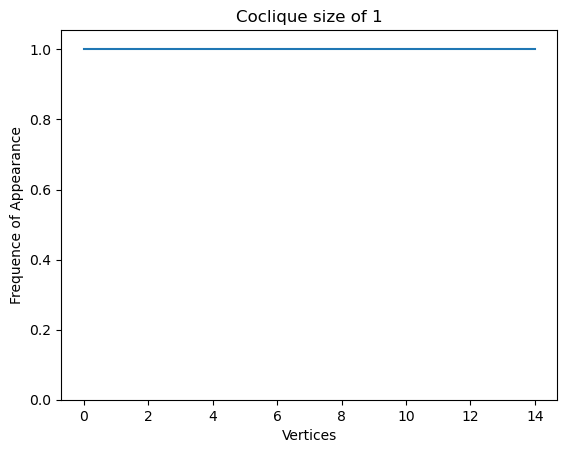
\includegraphics[width=1\linewidth]{images/depth_4_size_1.png}
			\caption{independent set of size 1}
		\end{subfigure}
		\begin{subfigure}[b]{.45\textwidth}
			\centering
			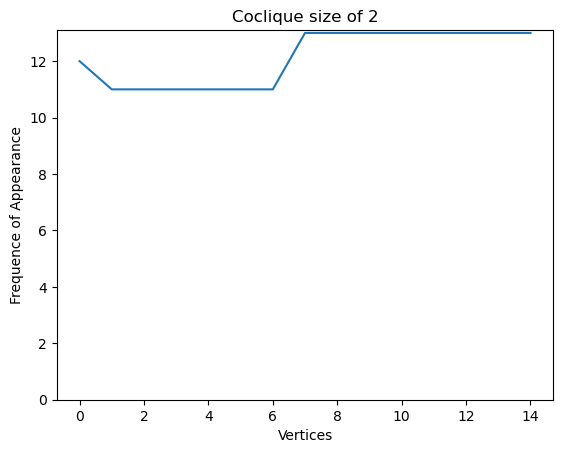
\includegraphics[width=1\linewidth]{images/depth_4_size_2.png}
			\caption{independent of size 2}
		\end{subfigure}
		\begin{subfigure}[b]{.45\textwidth}
			\centering
			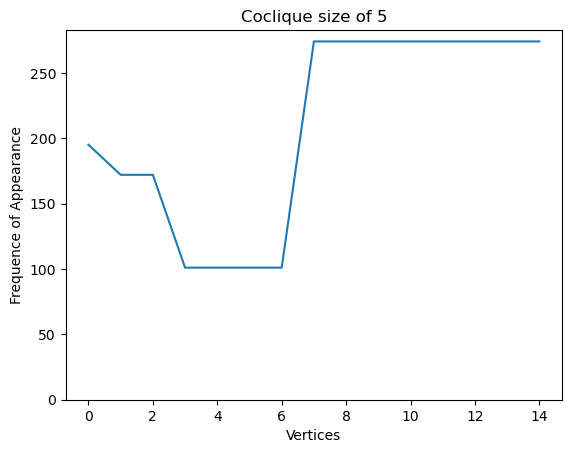
\includegraphics[width=1\linewidth]{images/depth_4_size_5.png}
			\caption{independent of size 5}
		\end{subfigure}
		\begin{subfigure}[b]{.45\textwidth}
			\centering
			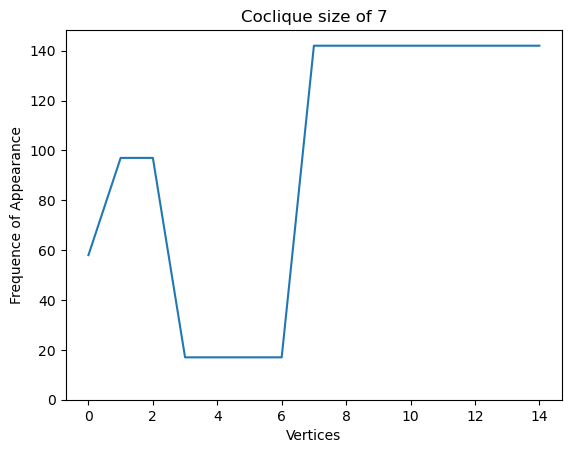
\includegraphics[width=1\linewidth]{images/depth_4_size_7.png}
			\caption{independent of size 7}
		\end{subfigure}
		\begin{subfigure}[b]{.45\textwidth}
			\centering
			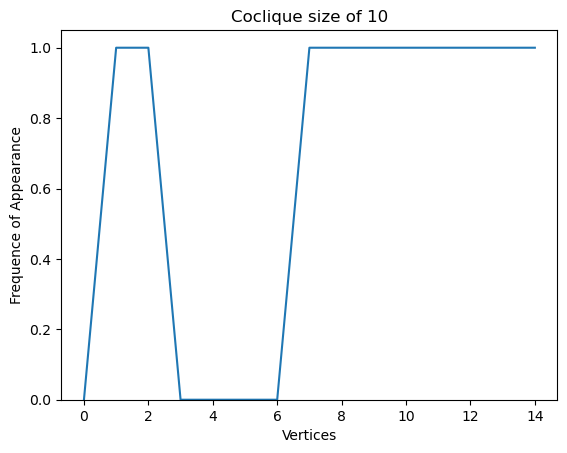
\includegraphics[width=1\linewidth]{images/depth_4_size_10.png}
			\caption{independent of size 10}
		\end{subfigure}
	\end{figure}

	\begin{figure}[hbt!]
		\caption*{Depth 5}
		\begin{subfigure}[b]{.45\textwidth}
			\centering
			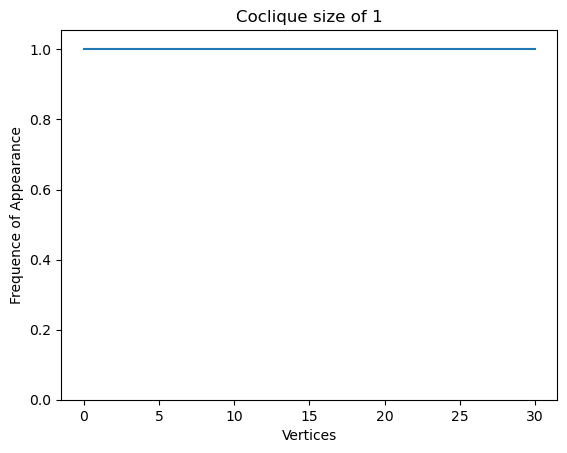
\includegraphics[width=1\linewidth]{images/depth_5_size_1.png}
			\caption{independent of size 1}
		\end{subfigure}
		\begin{subfigure}[b]{.45\textwidth}
			\centering
			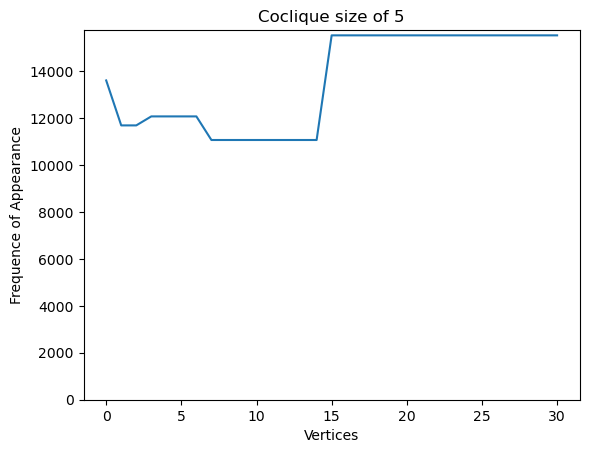
\includegraphics[width=1\linewidth]{images/depth_5_size_5.png}
			\caption{coclique of size 5}
		\end{subfigure}
		\begin{subfigure}[b]{.45\textwidth}
			\centering
			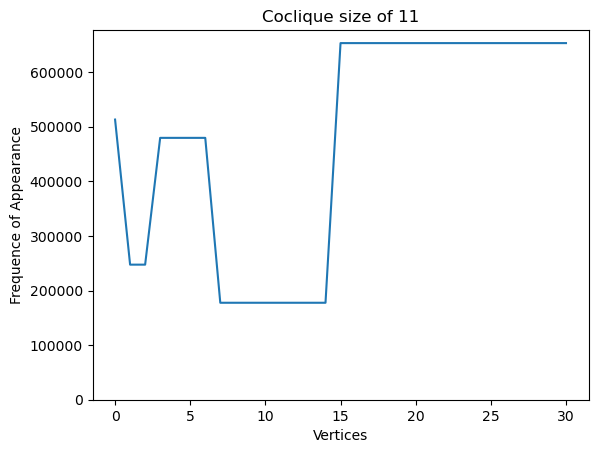
\includegraphics[width=1\linewidth]{images/depth_5_size_11.png}
			\caption{coclique of size 11}
		\end{subfigure}
		\begin{subfigure}[b]{.45\textwidth}
			\centering
			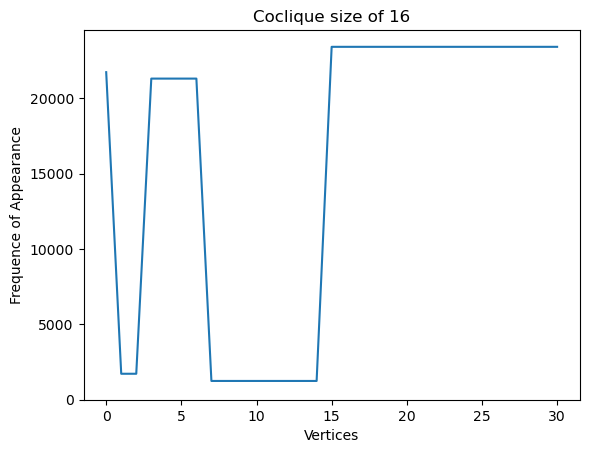
\includegraphics[width=1\linewidth]{images/depth_5_size_16.png}
			\caption{coclique of size 16}
		\end{subfigure}
		\begin{subfigure}[b]{.45\textwidth}
			\centering
			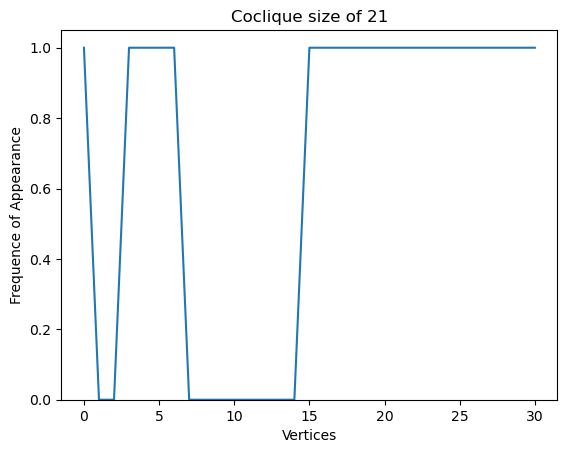
\includegraphics[width=1\linewidth]{images/depth_5_size_21.png}
			\caption{coclique of size 21}
		\end{subfigure}
	\end{figure}
	\newpage

	The data shown in the figures above verifies that the HK-Property holds for perfect binary trees of depth 5. The next step would be to verify this for perfect binary trees of depth 6 and 7.

	However, the algorithm is very slow and inefficient and it scales exponentially. Hence, running the algorithm for perfect binary trees of depth 6 and 7 would be very computationally expensive.

	\section{Generating Functions Algorithm and Analysis}\label{generating-functions-algorithm}

	To overcome the computational inefficiency of the brute force algorithm, we use generating functions to count the number of independent sets of a perfect binary tree of depth $d$. We then can compute the difference between the coefficients of the generated polynomials to determine if the HK-property holds for perfect binary trees numerically. 

	Recall from Lemma \ref{lemma:generating_def} that the polynomials $P_d, Q_d, R_d$ satisfy the following recurrent formulas for $n\geq 2$ with $P_{0}=1, P_1=1+x$, and $Q_{0}=0, Q_1=x$:
	\begin{align*}
		P_n(x) &= (P_{n - 1}(x))^2 + x(P_{n - 2}(x))^4  \\
		R_n(x) &= x(P_{n - 2}(x))^4  \\
		Q_n(x) &= Q_{n - 1}(x)P_{n - 1}(x) + xQ_{n - 2}(x)(P_{n - 2}(x))^3
	\end{align*}

	We present the following algorithm to generate the polynomials $P_d, Q_d, R_d$ for a perfect binary tree of depth $d$:

	\begin{algorithm}[H]
		\caption{Generate $P$ Sequence}
		\KwIn{$n$ (integer)}
		\KwOut{$P$ sequence}
		$P \gets [1, x+1]$\;
		\For{$i \gets 2$ \textbf{to} $n-1$}{
		    $P[i] \gets P[i-1]^2 + x \cdot P[i-2]^4$\;
		}
		\Return $P$
		\end{algorithm}

	\begin{algorithm}[H]
		\caption{Generate $Q$ Sequence}
		\KwIn{$n$ (integer)}
		\KwOut{$Q$ sequence}
		$Q \gets [0, x]$\;
		\For{$i \gets 2$ \textbf{to} $n-1$}{
		    $Q[i] \gets Q[i-1] \cdot P[i-1] + x \cdot Q[i-2] \cdot P[i-2]^3$\;
		}
		\Return $Q$
	\end{algorithm}

	\begin{algorithm}[H]
		\caption{Generate $R$ Sequence}
		\KwIn{$n$ (integer)}
		\KwOut{$R$ sequence}
		$R \gets [0, x]$\;
		\For{$i \gets 2$ \textbf{to} $n-1$}{
		    $R[i] \gets x \cdot P[i-2]^4$\;
		}
		\Return $R$
	\end{algorithm}

	\vspace{1cm}
	We then compare the coefficients of the polynomials $Q_d$ and $R_d$ to determine if the HK-property holds for perfect binary trees of depth $d$. The following algorithm checks if the HK-property holds for a given $P, Q, R$ sequence:
	\newline

	\begin{algorithm}[H]
		\caption{Check HK-Property}
		\KwIn{$P, Q, R$ sequences}
		\KwOut{Boolean}
		\For{$i \gets 2$ \textbf{to} $n-1$}{
		    \If{$Q[i] < R[i]$}{
		        \Return \textbf{False}
		    }
		}
		\Return \textbf{True}
	\end{algorithm}

\end{appendix}

\newpage
%______________________________________________________________
%~~~~~~~~~~~~~~~~~~~~~~~~~~~~~~~~~~~~~~~~~~~~~~~~~~~~~~~~~~~~~~

\include{Bibliography}
\bibliographystyle{plain}
\addcontentsline{toc}{chapter}{Bibliography}
\bibliography{Bibliography}

%______________________________________________________________
%~~~~~~~~~~~~~~~~~~~~~~~~~~~~~~~~~~~~~~~~~~~~~~~~~~~~~~~~~~~~~~
\end{document}

